\section{Methods}

\subsection{Data Collection}
For shape sensitivity analysis, representative 3D models of rTSA humeral and glenosphere implants, as well as TKA femoral and tibial implants, were obtained from a manufacturer.
The study focused on a single size for each implant type, as the scale of the shapes was normalized using an Invariant Shape Descriptor, rendering multiple sizes unnecessary for this analysis.
\subsection{Image Generation}
Each implant's binary silhouette was rendered to a $1024\times 1024$ image plane using an in-house CUDA camera model (CUDA Version 12.1) \cite{nickollsScalableParallelProgramming2008}.
The model featured a 1000mm focal length and 0.3mm per pixel resolution, which are quite typical projection parameters for fluoroscopic images.
All imaging tasks utilized an NVIDIA Quadro P2200 GPU.
\subsection{Invariant Angular Radial Transform}
The Invariant Angular Radial Transform Descriptor (IARTD) was selected for its radial direction sensitivity, enabling the detection of subtle contour changes in projected shapes \cite{leeNewShapeDescription2012}.
This sensitivity allows us to address minor changes along the contour of the projected shape, which is a desirable property for determining the minor changes in shape with respect to input orientation.

IARTD computation involves aggregating orthogonal basis components across the unit polar disk, forming a complex moment.
Each basis function has an order ($n$) and a repetition ($p$).
The order can be visualized as concentric rings on the polar disk, and the repetition as the count of slices partitioning the unit disk along $\theta$.
For these calculations, the image is normalized so that the center is at $(0,0)$, and the four corners are at $(\pm1,\pm1)$.

Each angular radial transform (ART) coefficient is a complex double integral (\cref{eq:F_np}) over the image in polar coordinates, $f(\rho,\theta)$ multiplied by the ART basis function, $V_{np}(\rho,\theta)$ (\cref{eq:V_np}).

\begin{equation}
	\label{eq:F_np}
	F_{np} = \int_{0}^{2\pi}\int_{0}^{1}f(\rho,\theta)V_{np}(\rho,\theta)\rho d\rho d\theta
\end{equation}

\begin{equation}
	\label{eq:V_np}
	V_{np}(\rho,\theta) = A_{p}(\theta)R_{n}(\rho)
\end{equation}

The radial basis function includes a complex exponential, $A_{p}(\theta)$ (\cref{eq:A_p}), ensuring rotational invariance, and a trigonometric transform, $R_{p}(\theta)$ (\cref{eq:R_n}), to establish orthogonality.

\begin{equation}
	\label{eq:A_p}
	A_{p}(\theta) = \dfrac{1}{2\pi}e^{jp\theta}
\end{equation}
\begin{equation}
	\label{eq:R_n}
	R_{n}(\rho) =
	\begin{cases}
		1                   & n=0     \\
		2 \cos (\pi n \rho) & n \ne 0
	\end{cases}
\end{equation}

Phase correction is applied to each ART coefficient (\cref{eq:art_phase_correction}, \cref{eq:fnp_phase_correction}) to adjust for differences in in-plane rotation.

\begin{equation}
	\label{eq:art_phase_correction}
	\phi'_{np} = \phi_{np} - \phi_{n,1}
\end{equation}

\begin{equation}
	\label{eq:fnp_phase_correction}
	F_{np}' = F_{np}e^{-jp\phi_{n,1}}
\end{equation}

Subsequently, the final feature vector is formulated by the polar decomposition of each coefficient at every order and repetition (\cref{eq:iartd}).
Values from the first two repetitions are excluded, as they do not provide significant information \cite{leeNewShapeDescription2012}.
The complete IARTD feature vector encompasses values of $n={0, \dots, 3 }$ and $p={0, \dots, 8}$ per the original authors' suggestion \cite{leeNewShapeDescription2012}.

\begin{equation}
	\label{eq:iartd}
	IARTD = \{|F'_{np}|, \phi_{np}'\} \text{ where } n \ge 0, p \ge 2
\end{equation}

\subsection{Shape Differences and Sensitivity}
In order to quantify the overall change between shapes, a readily interpretable value must be established.
To simplify notation, successive rotations are denoted as subscripts, with $R_{z}R_{x}R_{y}$ being represented as $R_{z,x,y}$.
If more than 3 rotations are applied successively, the full rotation sequence will be captured as $R_{r_{1},r_{2},r_{3},\cdots,r_{n}}$.
Similarly, the application of the IARTD equation to an implant at a specific input orientation $R_{z,x,y}$ is denoted as $IARTD(R_{z,x,y})$.
Shape differences were calculated using the central difference equation on the IARTD vector produced from two different orientations.
The grid of sampled orientations had extrema of $\pm 30^{\circ}$ with a step size of $5^{\circ}$ for each of the $x$, $y$, and $z$ axes.
The ``differences'' along each axis were computed using a positive and negative rotation ($\pm \delta $) of 1 degree .
Therefore, for every set of $x,y,z$ rotations, three distinct shape differences are computed, one each for $\delta_{x}$, $\delta_{y}$, and $\delta_{z}$ (\cref{eq:shape-derivative}).

\begin{figure}[h!]
  \centering
  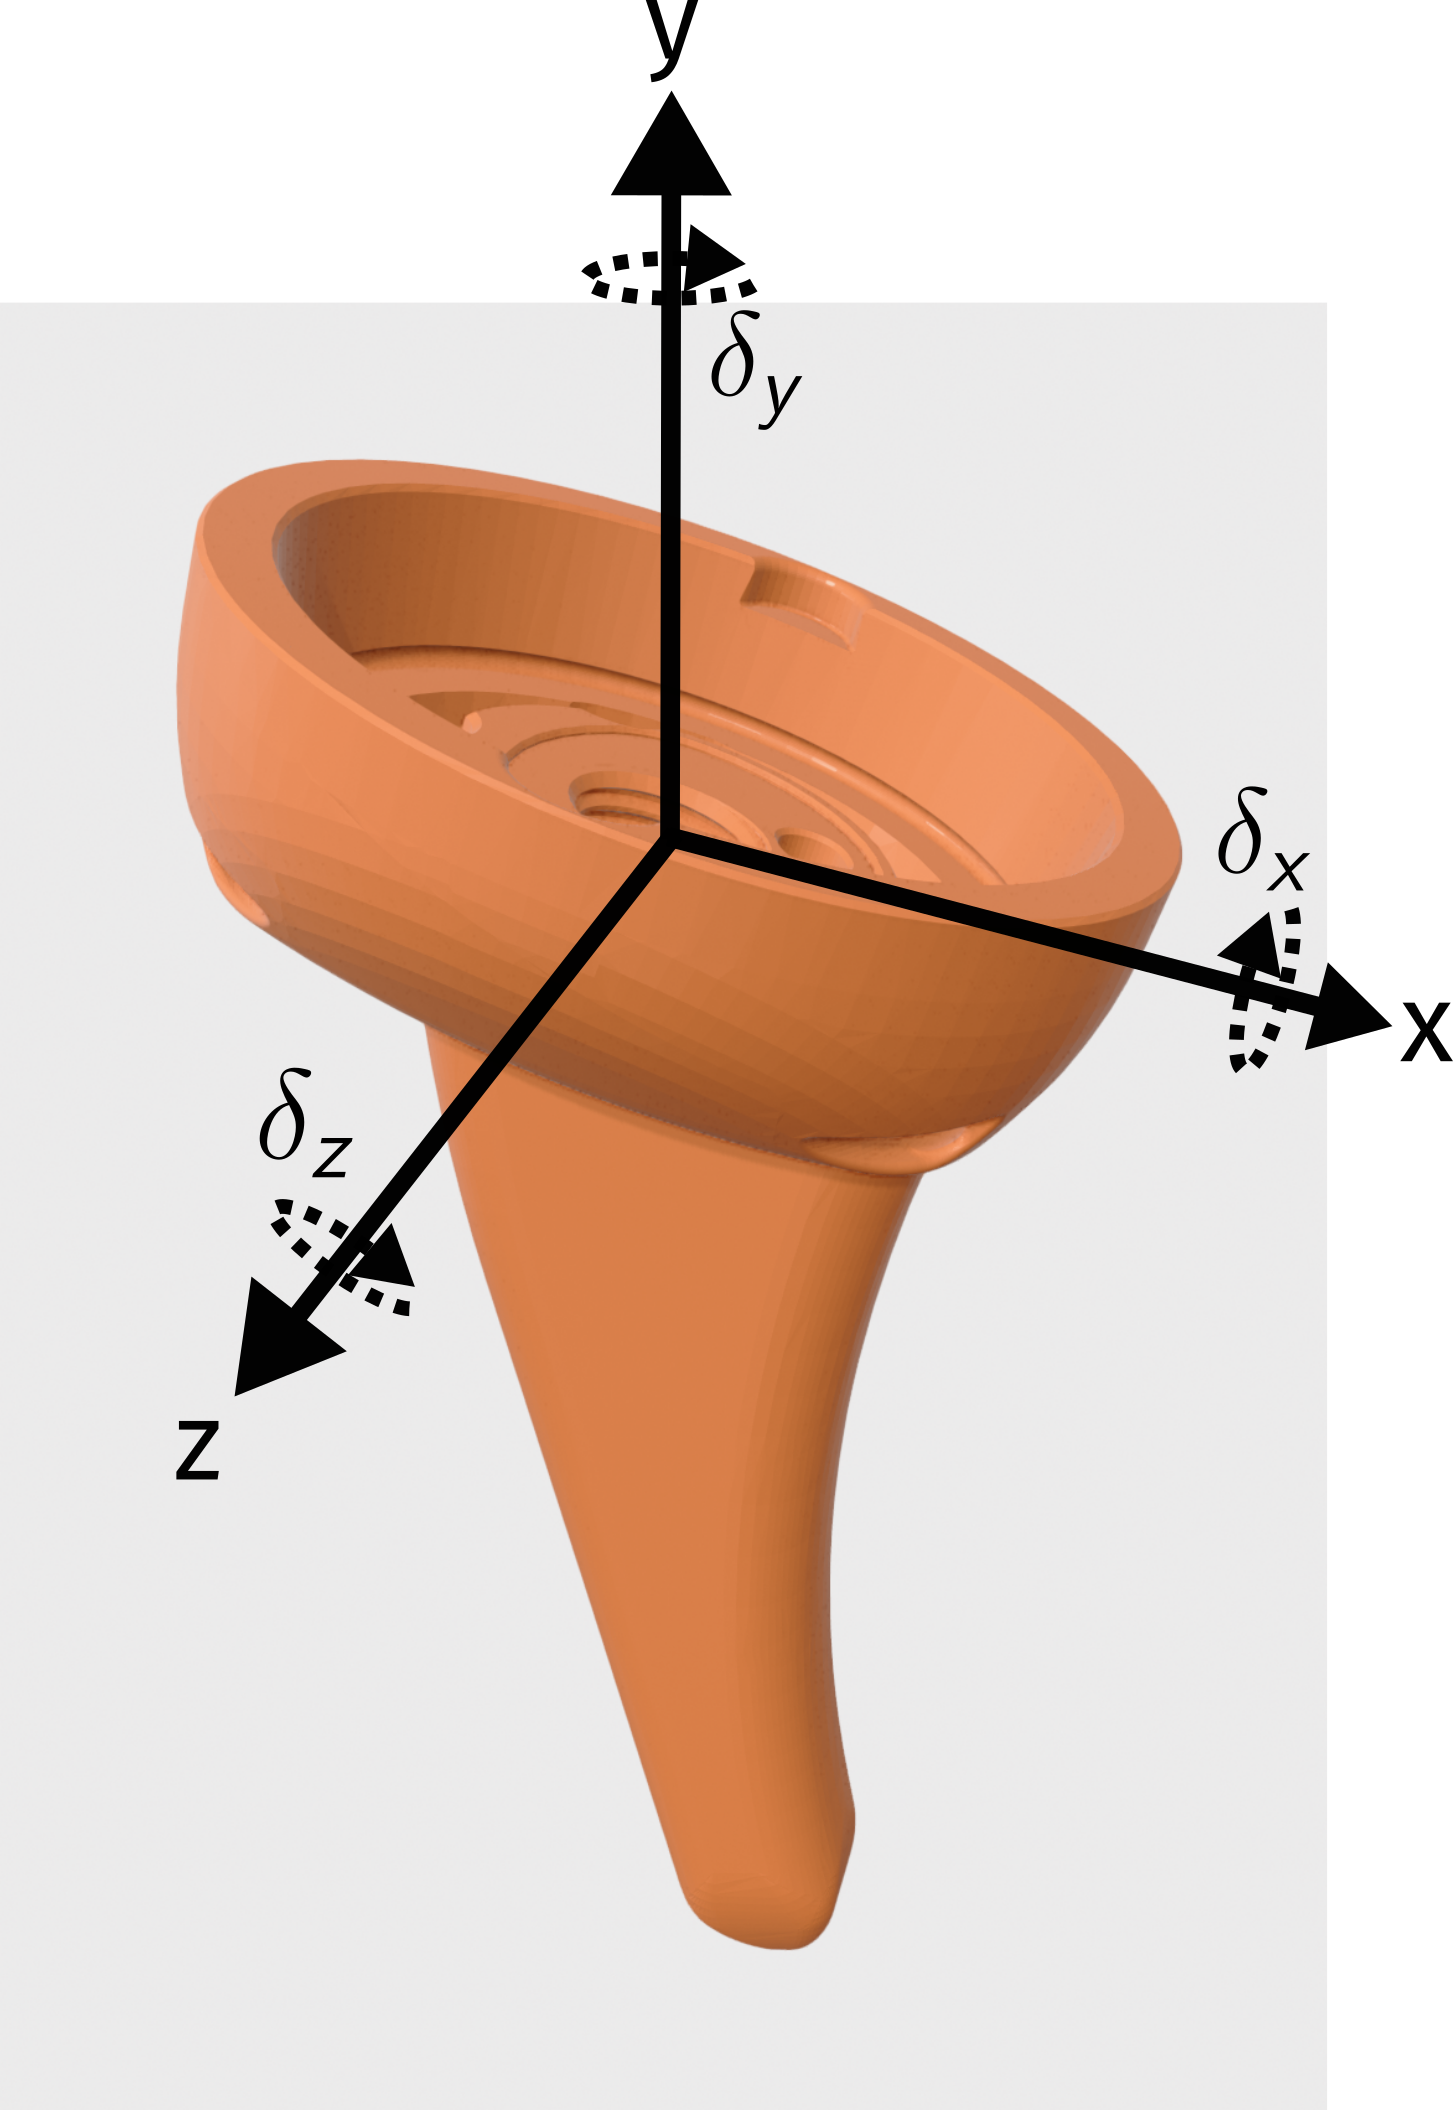
\includegraphics[width=0.5\textwidth]{rTSA_humeral_rotation_axes.png}
  \caption{A generic manufacturer-provided humeral implant with label x, y, and z rotation axis. Additionally, each of the ,$\delta_x$,$\delta_y$, and $\delta_z$ are shown, corresponding to the rotational directions of each shape descriptor difference.}
  \label{fig:rot-axis}
\end{figure}

For notational brevity, we will condense the total equation to a single $\Delta S(\delta)$, (representing $\Delta Shape$ for a differential rotation $\delta$).

\begin{equation}
	\label{eq:shape-derivative}
	\begin{split}
		\Delta S(\delta)_{z,x,y}  \equiv & IARTD(R_{z,x,y,+\delta})                        \\
		                                 & - IARTD(R_{z,x,y,-\delta})                      \\
		\forall                          & \delta \in \{\delta_{x},\delta_{y},\delta_{z}\}
	\end{split}
\end{equation}

The disparate scales of IARTD vector elements necessitate their normalization, ensuring a balanced assessment of global behavior without overemphasis on any individual element.
Z-scaling provides a practical approach to normalizing each element relative to its distribution.
After z-scaling, the Euclidean norm of each $S(\delta)_{z,x,y}$ is calculated to quantify the total shape change for a specific differential rotation (\cref{eq:euc_norm}).

The final step takes advantage of two factors: first, that the in-plane rotations are the first in the Euler sequence ($z$-axis), and second, that this type of rotation does not affect the in-plane shape.
For each $x$ and $y$ input rotation, an average is computed from values where $x$ and $y$ remain constant while $z$ varies (\cref{eq:z_rot_norm}). The final values are obtained from this equation, denoted by $\mathbb{S}$.
Individual plots were created for $\mathbb{S}_{x,y}$, corresponding to each differential rotation in $x$, $y$, and $z$, and for each of the four implant types.
An analysis of these plots were conducted to assess the performance of JTML optimization and to explore areas where low shape-sensitivity will pose significant challenges for registration-based optimization.

\begin{equation}
	\label{eq:euc_norm}
	\|S(\delta)_{z,x,y}\|_{2}
\end{equation}

\begin{equation}
	\label{eq:z_rot_norm}
	\mathbb{S}(\delta)_{x,y} = \dfrac{\sum_{z} \| S(\delta)_{z,x,y} \|_{2}}{N}
\end{equation}

%%% Local Variables:
%%% mode: latex
%%% TeX-master: "Jensen_Shape_Sensitivity"
%%% End:
